% Generated by render.py; edit preamble.tex and descendant.tikz
\documentclass[border=12pt]{standalone}
\def\pgfsysdriver{pgfsys-dvisvgm.def}
\usepackage[dvisvgm]{xcolor}
\usepackage{xeCJK}
\setCJKmainfont{HaranoAjiGothic-Regular.otf}[BoldFont=HaranoAjiGothic-Bold.otf]
\setCJKsansfont{HaranoAjiGothic-Regular.otf}[BoldFont=HaranoAjiGothic-Bold.otf]
\usepackage{amsmath,amssymb,tikz,lmodern}
\usetikzlibrary{arrows.meta,positioning,calc,fit,backgrounds}
\renewcommand{\familydefault}{\sfdefault}
\definecolor{ink}{HTML}{25322F}
\definecolor{green}{HTML}{246657}
\definecolor{tint}{HTML}{EEF4F0}
\definecolor{soft}{HTML}{C6D2CC}
\definecolor{muted}{HTML}{52615B}
\newif\ifJapanese
\newcommand{\Tx}[2]{\ifJapanese #1\else #2\fi}
\newcommand{\Eff}{\overline{\operatorname{Eff}}}
\newcommand{\heading}[3]{{\color{green}\bfseries #1\quad\Tx{#2}{#3}}\\[5pt]}
% A white rectangle makes the complete citation label clickable, including spaces.
\newcommand{\refurl}[2]{\special{dvisvgm:raw <a xlink:href="#1" target="_blank" rel="noopener noreferrer">}{\setlength{\fboxsep}{0pt}\colorbox{white}{\color{green}\underline{\strut #2}}}\special{dvisvgm:raw </a>}}
\tikzset{
 card/.style={draw=soft,fill=white,rounded corners=2pt,align=left,text=ink,font=\fontsize{10.5}{14}\selectfont,inner xsep=12pt,inner ysep=10pt,text width=14.4cm},
 half/.style={card,text width=6.45cm,minimum height=2.05cm},
 result/.style={card,draw=green,fill=tint,line width=.9pt},
 reason/.style={align=left,text=muted,font=\fontsize{9}{12}\selectfont,inner sep=0pt,text width=12.6cm},
 branchreason/.style={reason,text width=5.95cm},
 edge/.style={-{Stealth[length=2.4mm]},draw=green,line width=1pt},
 wire/.style={draw=green,line width=1pt},
}
% Keep the arrow in a dedicated left gutter; explanations never cover it.
\def\flow#1#2#3;{
 \coordinate (#2-from) at ($(#1.south)+(-6.9,0)$);
 \coordinate (#2-to) at ($(#2.north)+(-6.9,0)$);
 \draw[edge] (#2-from)--(#2-to);
 \node[reason,anchor=west] (#2-reason) at ($(#2-from)!.5!(#2-to)+(.55,0)$) {#3};
}

% Style adapted from the repository's Schnell diagrams; MIT attribution retained.
\newcommand{\PRef}[1]{\refurl{https://github.com/openai/math/blob/fd4aeeb2ee4fc729c18d98444fed42fd0529eeeb/preprints/The-Generalized-Mukai-Conjecture-September-24-2026/article.pdf}{#1}}
\newcommand{\MMRef}[1]{\refurl{https://arxiv.org/pdf/math/0409569v4\string##page=5}{#1}}
\newcommand{\TZRef}[1]{\refurl{https://arxiv.org/pdf/1209.4342v5\string##page=4}{#1}}
\newcommand{\KMRef}[1]{\refurl{https://www.ihes.fr/~maxim/TEXTS/relation_between_23.pdf\string##page=7}{#1}}
\newcommand{\PARef}[1]{\refurl{https://www.numdam.org/item/SB_1997-1998__40__307_0.pdf\string##page=6}{#1}}
\newcommand{\BCRef}[1]{\refurl{https://druel.perso.math.cnrs.fr/textes/mukai.pdf\string##page=23}{#1}}
\newcommand{\ERRef}[1]{\refurl{https://druel.perso.math.cnrs.fr/textes/mukai_erratum.pdf}{#1}}
\newcommand{\OCRef}[1]{\refurl{https://doi.org/10.4153/CMB-2006-028-3}{#1}}

\Japanesefalse
\begin{document}
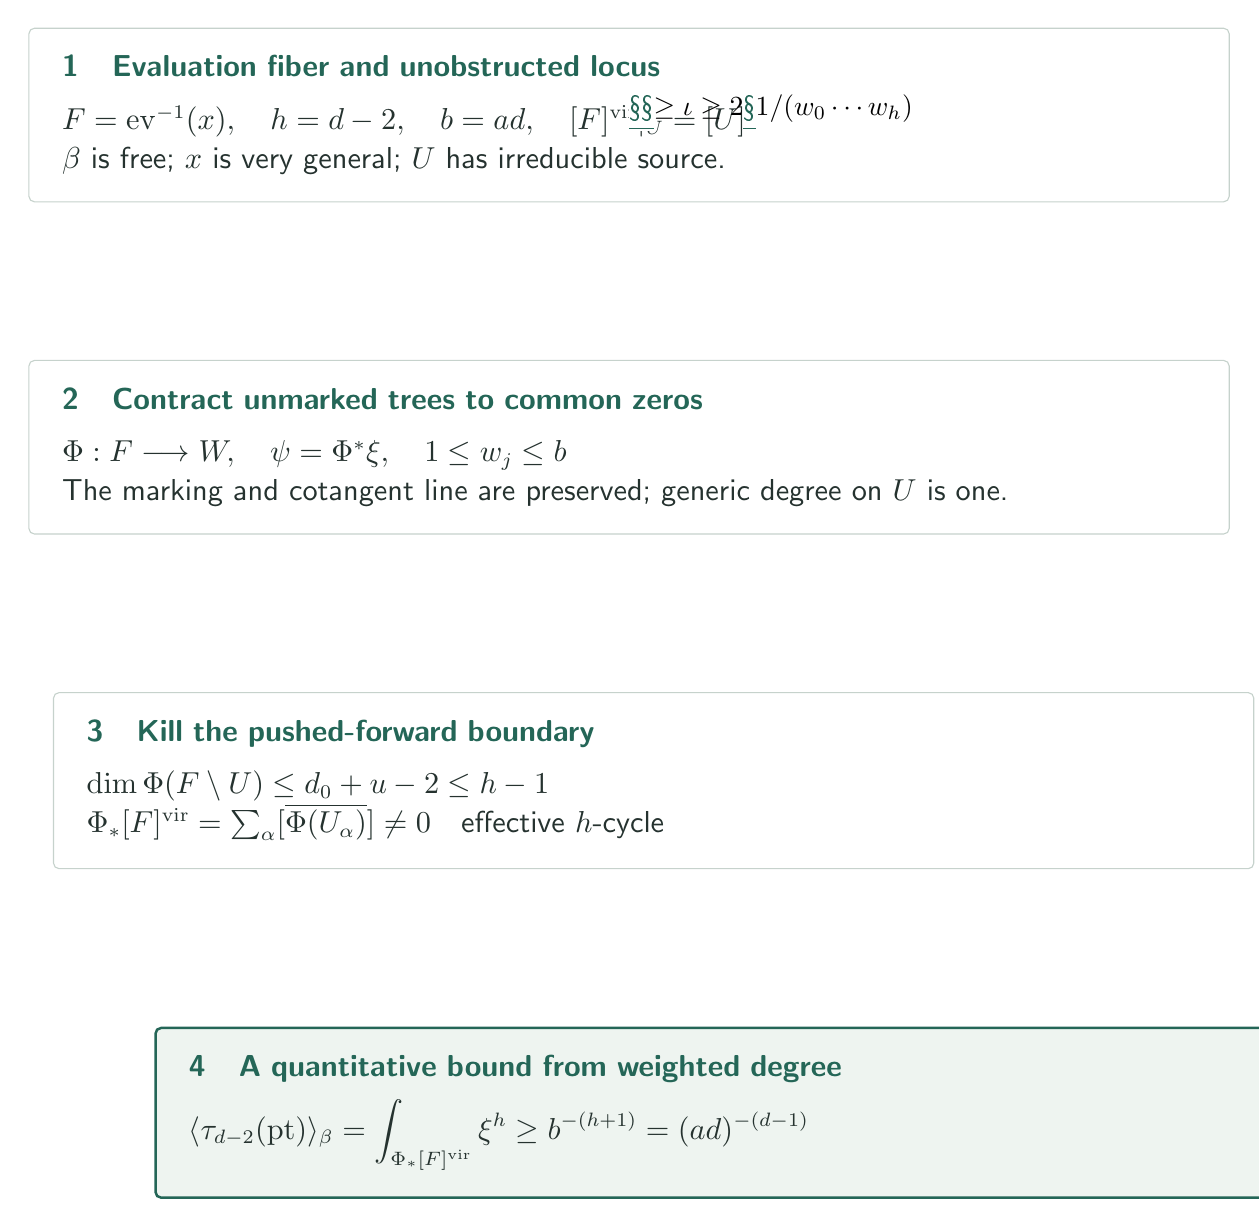
\begin{tikzpicture}

\node[card] (a) {\heading{1}{評価ファイバーと非障害部分}{Evaluation fiber and unobstructed locus}
$F=\mathrm{ev}^{-1}(x),\quad h=d-2,\quad b=ad,\quad [F]^{\mathrm{vir}}|_U=[U]$\\
\Tx{$\beta$ は free、$x$ は非常に一般、$U$ は既約な源を持つ写像}{$\beta$ is free; $x$ is very general; $U$ has irreducible source.}};
\node[card,below=2cm of a] (b) {\heading{2}{印以外を共通零点へ縮約}{Contract unmarked trees to common zeros}
$\Phi:F\longrightarrow W,\quad \psi=\Phi^*\xi,\quad 1\le w_j\le b$\\
\Tx{印の近傍と cotangent line を保ち、$U$ 上の generic degree は1}{The marking and cotangent line are preserved; generic degree on $U$ is one.}};
\flow{a}{b}{\Tx{全次数を印の成分へ移す：}{Move all degree to the marked component: }\PRef{\S\S3.2--3.3, pp. 7--8}\\
\MMRef{Intermediate moduli, Prop. 1.3, pp. 5--6}\ \Tx{（別構成）}{(alternative construction)}};
\node[card,below=2cm of b] (c) {\heading{3}{境界の押し出しを消す}{Kill the pushed-forward boundary}
$\dim\Phi(F\setminus U)\le d_0+u-2\le h-1$\\
$\Phi_*[F]^{\mathrm{vir}}=\sum_\alpha[\overline{\Phi(U_\alpha)}]\ne0$\quad\Tx{有効 $h$-cycle}{effective $h$-cycle}};
\flow{b}{c}{\Tx{各 tail の次数 $\ge\iota\ge2$、Chow localization：}{Each tail has degree $\ge\iota\ge2$; Chow localization:}\\
\PRef{\S3.4, pp. 8--9}\quad\Tx{仮想類そのものの有効性は不要}{No effectivity of the virtual class itself is used.}};
\node[result,below=2cm of c] (d) {\heading{4}{重み付き次数から定量的下界}{A quantitative bound from weighted degree}
$\displaystyle \langle\tau_{d-2}(\mathrm{pt})\rangle_\beta
=\int_{\Phi_*[F]^{\mathrm{vir}}}\xi^h\ge b^{-(h+1)}=(ad)^{-(d-1)}$};
\flow{c}{d}{\Tx{座標部分スタックの次数 $1/(w_0\cdots w_h)$ と射影公式：}{Coordinate-substack degree $1/(w_0\cdots w_h)$ and projection formula:}\\
\PRef{Lemma 3.2; Prop. 3.1, pp. 9--10}};

\end{tikzpicture}
\end{document}
